\section*{Simuleringer}
Efter at indgangsvælgeren er blevet designet og beregnet, er det lavet en række simuleringer for se om kredsløbet opfører sig som ønsket og, hvis der er afvigelser, give en begrundelse for hvorfor. I dette afsnit vil der blive simuleret følgende Dæmpning af signal, THD, frekvenskarakteristik, forstærkning igennem kredsløbet, tænd og sluk af signal. Det samlede diagram der er simuleret kan ses på figur \ref{diagram_simulering}. Alle simuleringen er udført med et input på 2 V peak og 1 kHz, hvis ikke andet er anført.

\begin{figure}[h]
\centering
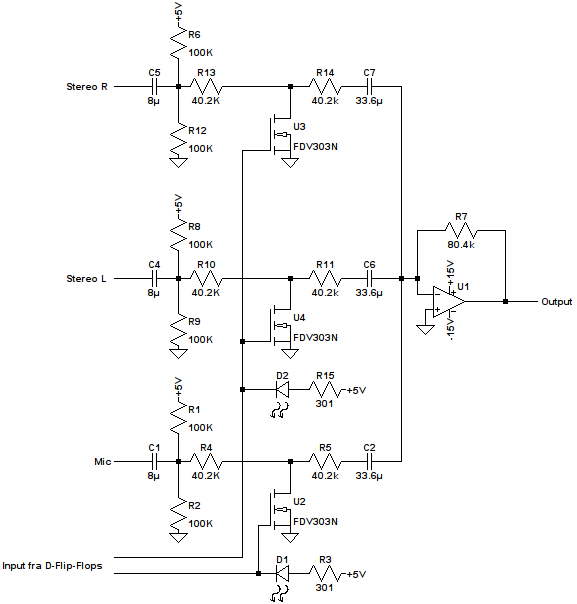
\includegraphics[scale=0.4]{teknisk/indgangsvaelger/simulering/indgangvaelger_ltspice_diagram.png}
\caption{Diagram over det kredsløb der simuleres.}
\label{diagram_simulering}
\end{figure}

\subsection*{Forstærkning igennem kredsløbet}
Fra beregningerne vides det at kredsløbet er designet til at have en forstærkning på 1. Derudover vil signalet efter indgangsvælgeren også være inverteret. Det simulerede signal er vist på figur \ref{indgangsvaelger_input/output}.
\begin{figure}[h]
\centering
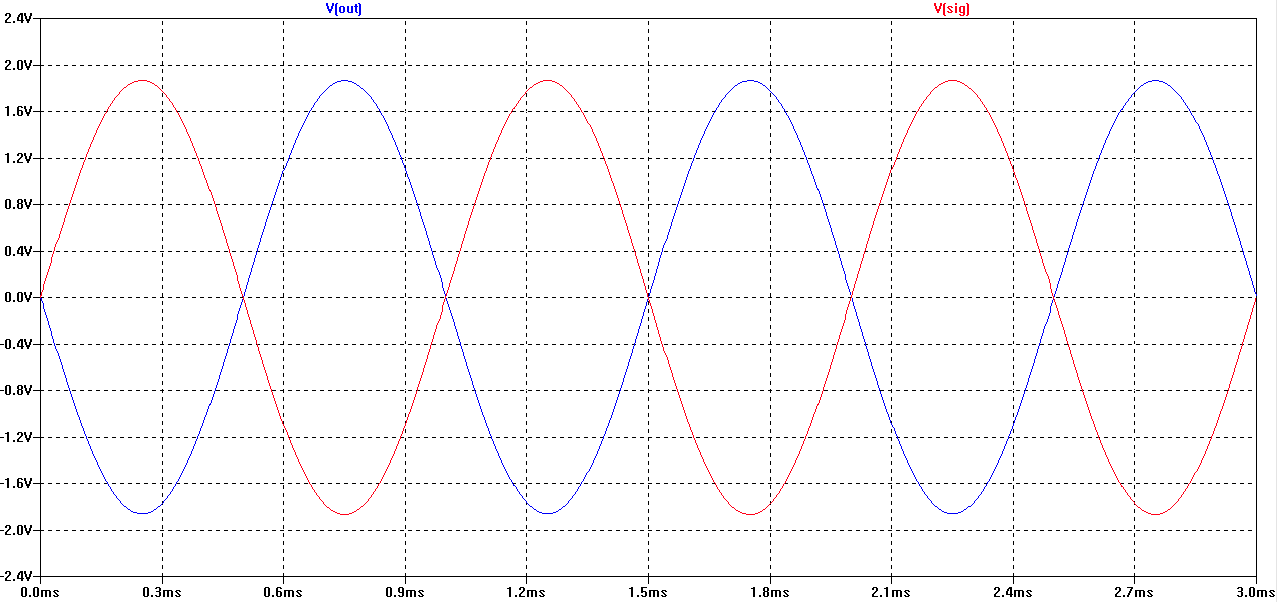
\includegraphics[scale=0.3]{teknisk/indgangsvaelger/simulering/input_output.png}
\caption{Forstærkningen igennem indgangsvælgeren. Den røde kurve inputsignalet til indgangsvælgeren og den blå er outputsignalet fra indgangsvælgeren.}
\label{indgangsvaelger_input/output}
\end{figure}

Som det ses på figur \ref{indgangsvaelger_input/output} er forstærkningen på 1 opnået og signalet er inverteret som forventet.


\subsection*{Frekvenskarakteristik}
På figur \ref{indgangsvaelger_frekvenskarakteristik} er simuleringen af frekvenskarakteristikken vist. Fra kravspecifikation er der opsat krav om at i frekvensområdet fra 20 Hz til 20 kHz må afvigelsen højest være $\pm$ 1.5 dB. På simuleringen ses det at fra 10 kHz til 20 kHz er der en lille afvigelse på ca. 0.06 dB, Dette skyldes at transistoren der er brugt har en passiv kapacitet der gør at ved høje frekvenser vil signalet falde af. Dette har dog ikke nogen betydning idet at forstærkeren i dette projekt ikke skal arbejde over 20 kHz.

\begin{figure}[h]
\centering
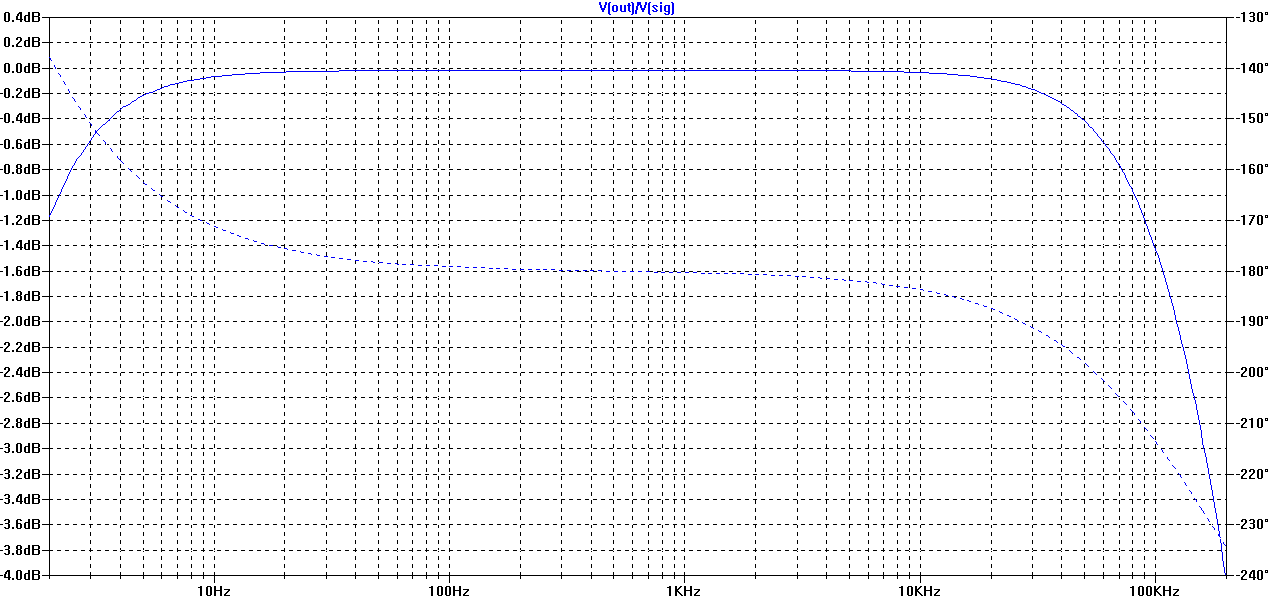
\includegraphics[scale=0.3]{teknisk/indgangsvaelger/simulering/frekvenskarakteristik.png}
\caption{Frekvens- og fasekarakteristikken for indgangsvælgeren.}
\label{indgangsvaelger_frekvenskarakteristik}
\end{figure}

\subsection*{Dæmpning af signal}
Fra kravspecifikationen er der opsat krav om at isoleringen af signaler skal være større end 50 dB. På figur \ref{indgangsvaelger_daempniing} ses en graf over hvor stor en dæmpning er simuleret til i kredsløbet. Dæmpningen er aflæst til minimum 89 dB, og er derfor accepteret.
\begin{figure}[h]
\centering
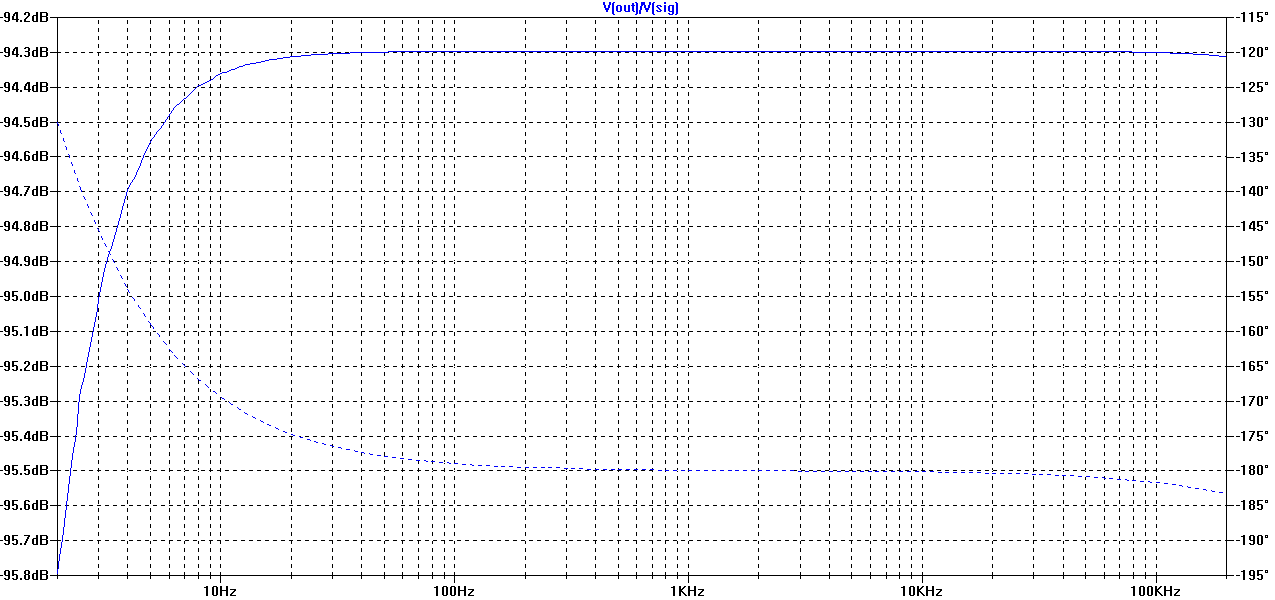
\includegraphics[scale=0.3]{teknisk/indgangsvaelger/simulering/daempning_af_signal.png}
\caption{Dæmpningsgraden af signalet, når det er slukket.}
\label{indgangsvaelger_daempniing}
\end{figure}

\subsection*{Tænd og sluk af signal}
På figur \ref{indgangsvaelger_taendsluk} er der simuleret at en signal bliver tændt og slukket. Denne simulering er lavet ved 100 Hz for at gøre det mere tydeligt at se det er et sinussignal. Som det ses er signalet når det bliver tændt ca. 700 ms om at komme op på det rigtige niveau. Dette skyldes at der er brugt kondensatorer til at fjerne DC spænding. Denne lange indsvingning af signalet vil bevirke at når det tændes vil et give et klik. 
\begin{figure}[h]
\centering
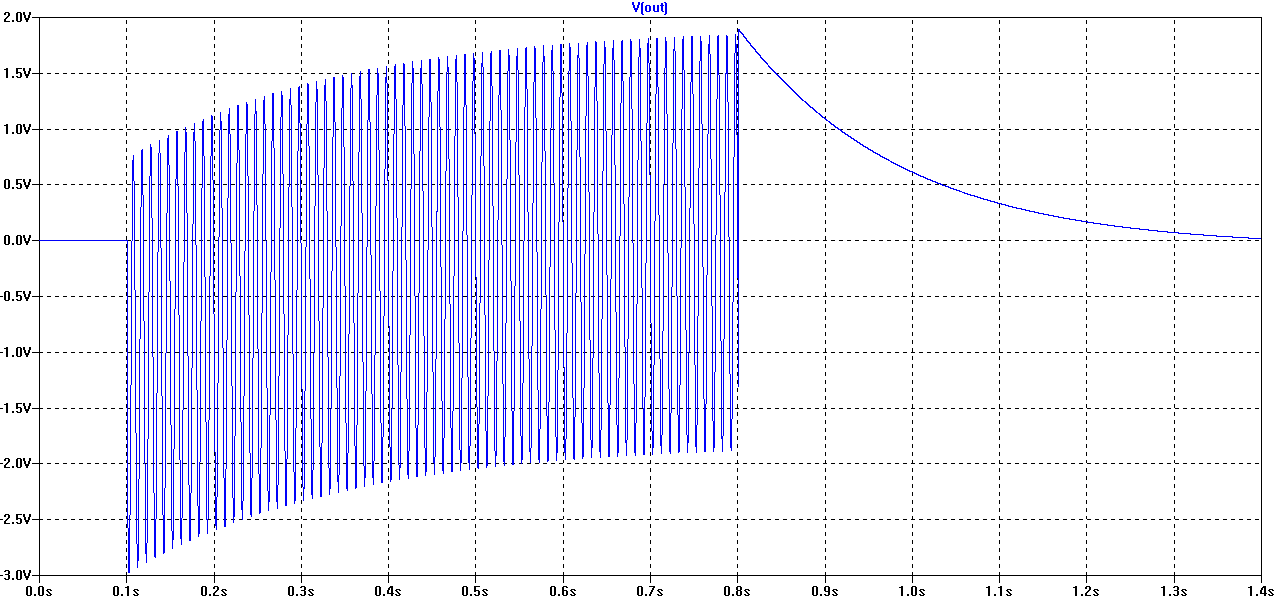
\includegraphics[scale=0.3]{teknisk/indgangsvaelger/simulering/taend_sluk.png}
\caption{Simulering af at tænde og slukke signalet.}
\label{indgangsvaelger_taendsluk}
\end{figure}